\section{随机变量}
\label{sec:rvd-random-variables}

掷一枚骰子，样本空间是$\Omega=\{1,2,3,4,5,6\}$。如果关心点数，就把结果$\omega$记成数$\omega$；如果只关心奇偶，就把偶数结果记成$1$、奇数结果记成$0$。两种记录面对的是同一次试验，区别只在于“结果怎样变成数”。这种记录规则怎样精确表述，它取各个值的概率又怎样从结果的概率得到？

\paragraph{结果到数值的映射}
图~\ref{fig:rvd-die-maps}画出了两种记录。中间一行是六个结果，向上的箭头把每个结果送到它的点数，向下的箭头把三个偶数结果送到$1$、三个奇数结果送到$0$。两种记录都是从$\Omega$到实数的函数，只是第二个函数把不同的结果合并到了同一个值。

\begin{BookInlineFigure}
  \centering
  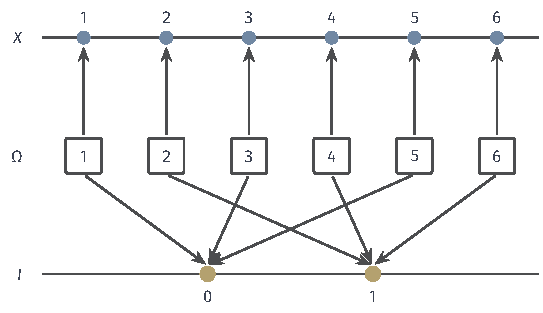
\includegraphics[width=92mm]{figures/07-probability/01-elementary-probability/tikz/rvd-die-maps/figure.pdf}
  \caption{同一次掷骰上的两个随机变量。中间一行是样本空间$\Omega$的六个结果。向上的箭头是点数$X$，六个结果送到六个不同的值（蓝点）；向下的箭头是奇偶记录$I$，三个奇数结果都送到$0$，三个偶数结果都送到$1$（黄点）。}
  \label{fig:rvd-die-maps}
\end{BookInlineFigure}

把这种规则一般地写出来，就得到随机变量。它的定义只用到样本空间和函数，概率在下一步才进入。

\begin{definition}[随机变量]
\label{def:rvd-random-variable}
设$\Omega$是一个试验的样本空间。函数$X:\Omega\to\mathbb{R}$称为\term{随机变量}（random variable）。对实数集的子集$B$，记
\begin{equation}
  \{X\in B\}=\{\omega\in\Omega:X(\omega)\in B\},
  \label{eq:rvd-preimage}
\end{equation}
它是由满足$X(\omega)\in B$的结果组成的事件，其概率记作$\mathbb{P}(X\in B)$。
\end{definition}

常用的事件有简写：$\{X\leq x\}$表示$B=(-\infty,x]$，$\{X=x\}$表示$B=\{x\}$，$\{a<X\leq b\}$表示$B=(a,b]$。在骰子的例子里，点数记录是$X(\omega)=\omega$，奇偶记录是
\[
  I(\omega)=\begin{cases}1,&\omega\in\{2,4,6\},\\0,&\omega\in\{1,3,5\}.\end{cases}
\]
于是$\{I=1\}=\{2,4,6\}$，$\{X\leq 2\}=\{1,2\}$，它们都是$\Omega$的子集，也就是第~\ref{chap:classical-probability}章意义下的事件。

一般地，对事件$A$，在$A$上取$1$、在$A$外取$0$的函数记作$\mathbf{1}_{A}$，称为$A$的\term{指示函数}（indicator function）。奇偶记录就是$I=\mathbf{1}_{\{2,4,6\}}$。指示函数把事件和随机变量联系起来：$\{\mathbf{1}_{A}=1\}=A$，所以$\mathbb{P}(\mathbf{1}_{A}=1)=\mathbb{P}(A)$。事件可以看成只取$0$和$1$的随机变量。

\paragraph{随机变量、实现值与事件}
“随机变量”这个名字容易误导：$X$本身是一个完全确定的函数，随机的是哪个结果$\omega$出现。试验做完，结果$\omega$确定，$X$就取一个具体的数$x=X(\omega)$，称为$X$的一个\term{实现值}（realization）。我们用大写字母表示随机变量，小写字母表示它的取值。

三种对象要分清。$X$是规则，在试验之前就已给定；$\{X\leq 2\}$是事件，是一个由结果组成的集合，事先可以问它的概率；“这次掷出$x=5$”是一次实现，事后才知道。说“$\mathbb{P}(X\leq 2)=1/3$”是在谈事件，说“$x=5>2$，所以事件$\{X\leq2\}$这次没有发生”是在用实现值检验事件。

\paragraph{由结果的概率得到取值的概率}
骰子公平时，每个结果的概率是$1/6$。要算$I$取$1$的概率，就把被送到$1$的结果的概率加起来：
\[
  \mathbb{P}(I=1)=\mathbb{P}(\{2,4,6\})=\tfrac16+\tfrac16+\tfrac16=\tfrac12 .
\]
可以把$\mathbb{P}$想成单位质量在六个结果上的分配，每个结果分到$1/6$。随机变量沿箭头把每个结果的质量搬到它的取值上，同一个取值收到的质量相加。$X$把六份质量分别搬到$1,\dots,6$，$I$把三份搬到$0$、三份搬到$1$。

同一个函数配上不同的概率，搬运的结果就不同。设骰子被做了手脚，$\mathbb{P}(\{6\})=1/2$，其余五面各为$1/10$。函数$I$没有变，但
\[
  \mathbb{P}(I=1)=0.1+0.1+0.5=0.7 .
\]
所以随机变量取值的概率规律由两样东西共同决定：结果到数值的规则$X$，以及结果上的概率$\mathbb{P}$。

\paragraph{无限多个结果}
等待时间可以是任何非负实数，样本空间$\Omega=[0,\infty)$有无穷多个结果，第~\ref{chap:classical-probability}章的计数比不再适用。本部分对这类试验直接规定区间事件的概率：例如规定等待超过$t$分钟的概率，再由加减得到其他区间的概率。具体的规定方式由下一节的分布函数和第~\ref{sec:rvd-mass-density}节的密度给出。

这样做时只对区间及其有限并谈概率，对取有限或可数个值的变量则对取值的任意子集谈概率。一般样本空间上哪些集合可以赋予概率、怎样保证各种规定彼此相容，在第~\ref{chap:probability-spaces}章统一处理。本部分用到的事件都是上面这些具体的集合，不会遇到困难。

\paragraph{同一次试验的不同记录}
同一次试验可以同时定义许多随机变量。掷两枚骰子，样本空间是$36$个等可能的有序对$\omega=(i,j)$。记点数之和为$S(\omega)=i+j$，较大的点数为$M(\omega)=\max\{i,j\}$。两者都是$\Omega$上的函数，记录的是同一次投掷的不同侧面。

事件$\{S=7\}$由反对角线上的六个结果组成，所以$\mathbb{P}(S=7)=6/36$。事件$\{M=4\}$由“较大者恰为$4$”的结果组成：$(4,1),\dots,(4,4)$与$(1,4),(2,4),(3,4)$，共$7$个，所以$\mathbb{P}(M=4)=7/36$。图~\ref{fig:rvd-two-dice}(a)用圆点和方框标出了这两个事件，$(3,4)$和$(4,3)$同时属于两者。

\begin{BookInlineFigure}
  \centering
  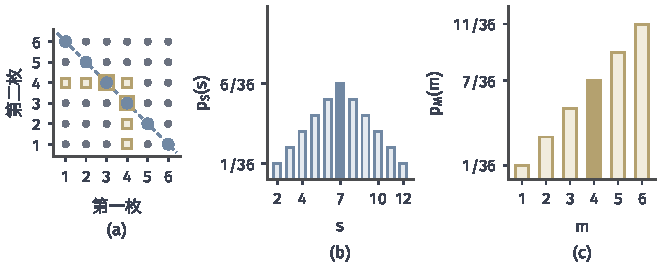
\includegraphics[width=112mm]{figures/07-probability/01-elementary-probability/matplotlib/rvd-two-dice/figure.pdf}
  \caption{两枚公平骰子上的两个随机变量。(a)$36$个等可能结果，蓝色圆点（沿虚线）是事件$\{S=7\}$，黄色方框是事件$\{M=4\}$，两个结果同时属于二者。(b)点数之和$S$取各值的概率，深色柱是$s=7$。(c)较大点数$M$取各值的概率，深色柱是$m=4$。}
  \label{fig:rvd-two-dice}
\end{BookInlineFigure}

对每个取值都这样计数，就得到图~\ref{fig:rvd-two-dice}(b)(c)。和为$s$的结果沿一条反对角线排列，条数先增后减，于是
\begin{equation}
  \mathbb{P}(S=s)=\frac{6-\lvert s-7\rvert}{36},\qquad s=2,3,\dots,12 .
  \label{eq:rvd-dice-sum}
\end{equation}
较大点数先用累计事件计数更方便：$\{M\leq m\}$要求两枚骰子都不超过$m$，有$m^{2}$个结果。$\{M=m\}$是$\{M\leq m\}$去掉$\{M\leq m-1\}$，所以
\[
  \mathbb{P}(M=m)=\frac{m^{2}-(m-1)^{2}}{36}=\frac{2m-1}{36},\qquad m=1,\dots,6 .
\]
两张表的概率各自加起来都等于$1$。

两个记录来自同一次投掷，彼此并不无关。知道$M=1$，就只能是$(1,1)$，于是$S=2$。这种同时考察多个随机变量的问题由第~\ref{chap:random-vectors}章处理，本章每次只看一个随机变量。

\paragraph{分布}
算出$\mathbb{P}(S=s)$之后，回答“$S$落在某个范围的概率”就不再需要回到$36$个结果：例如$\mathbb{P}(S\geq 10)=(3+2+1)/36=1/6$。我们只关心一个随机变量本身时，需要的正是这种“取值落在哪里、概率多大”的规律。

\begin{definition}[分布]
\label{def:rvd-distribution}
随机变量$X$的\term{分布}（probability distribution）是对实数集的子集$B$给出概率的规则
\begin{equation}
  P_X(B)=\mathbb{P}(X\in B)=\mathbb{P}(\{\omega\in\Omega:X(\omega)\in B\}).
  \label{eq:rvd-distribution}
\end{equation}
本部分中$B$取区间及其有限并；$X$只取有限或可数个值时，$B$可取这些值组成的任意集合。
\end{definition}

按搬运质量的图景，$\mathbb{P}$是单位质量在样本空间上的分配，$P_X$是这些质量被$X$搬到实轴之后的分配。分布只记录质量最后停在哪里，不再记录它从哪个结果搬来。这既是分布的用处，也是它的局限：凡是只涉及$X$一个变量取值的概率问题，分布都能回答；凡是涉及“哪个结果产生了这个值”的问题，分布无能为力。

\paragraph{分布本身也是概率}
$P_X$满足第~\ref{chap:classical-probability}章概率的基本规则，只是它作用在实数集的子集上，而不是$\Omega$的子集上。原因在于取原像与集合运算可以交换次序。对实数集的子集$B_1,B_2$，结果$\omega$属于$\{X\in B_1\cup B_2\}$，当且仅当$X(\omega)$落在$B_1$或$B_2$中，即$\omega$属于两个事件之一，所以
\[
  \{X\in B_1\cup B_2\}=\{X\in B_1\}\cup\{X\in B_2\}.
\]
同理，$\{X\notin B\}$是事件$\{X\in B\}$在$\Omega$中的补。

若$B_1$与$B_2$不相交，没有哪个结果能让$X(\omega)$同时落在两者中，两个事件互斥。由概率的可加性，
\[
  P_X(B_1\cup B_2)=P_X(B_1)+P_X(B_2).
\]
再加上$P_X(B)\geq0$和$P_X(\mathbb{R})=\mathbb{P}(\Omega)=1$，$P_X$就是实轴上的一个概率分配。此后只研究$X$时，可以把取值的集合当作新的样本空间，忘掉原来的$\Omega$。

新的样本空间上的概率通常不再是等可能的。两枚骰子的$36$个结果等可能，但点数之和的$11$个取值概率各不相同，式~\eqref{eq:rvd-dice-sum}中$7$的概率是$2$的六倍。在取值集合$\{2,\dots,12\}$上直接“数有利取值”会得出错误答案，这正是第~\ref{chap:classical-probability}章强调的：把基本结果合并之后，不能继续把合并后的类别当作等可能。

\paragraph{相同分布不等于相同取值}
在公平骰子上再定义$Y(\omega)=7-\omega$，即骰子底面的点数。$X$和$Y$在每个结果上都不相等，因为$X(\omega)=Y(\omega)$要求$\omega=3.5$。但$Y$取每个值$k$的概率是
\[
  \mathbb{P}(Y=k)=\mathbb{P}(\{7-k\})=\tfrac16,\qquad k=1,\dots,6,
\]
与$X$完全相同。图~\ref{fig:rvd-same-law}(a)逐个结果画出两个取值，(b)画出两者取各值的概率。

\begin{BookInlineFigure}
  \centering
  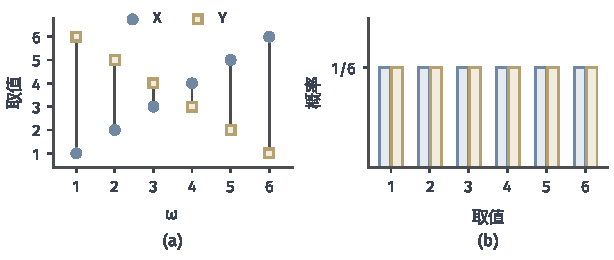
\includegraphics[width=104mm]{figures/07-probability/01-elementary-probability/matplotlib/rvd-same-law/figure.pdf}
  \caption{分布相同而取值不同。公平骰子上，$X(\omega)=\omega$（蓝点）与$Y(\omega)=7-\omega$（黄框）。(a)每个结果上两者的取值，竖线连接同一结果的两个值，没有一个结果使二者相等；(b)两者取$1,\dots,6$的概率都是$1/6$。}
  \label{fig:rvd-same-law}
\end{BookInlineFigure}

若$P_X=P_Y$，即对所有$B$都有$\mathbb{P}(X\in B)=\mathbb{P}(Y\in B)$，就说$X$与$Y$\term{同分布}（identically distributed）。同分布只是说两个变量“单独看”无法区分，不是说它们相等。这个例子里$X+Y$恒等于$7$，但仅凭两个分布无法知道这一点：若把$Y$换成另一枚独立骰子的点数，两个分布照旧，$X+Y$却会取$2$到$12$之间的各种值。表~\ref{tab:rvd-three-objects}总结了三个对象的区别。

\begin{BookInlineTable}
  \centering
  \begin{tabular}{lll}
    \toprule
    对象 & 是什么 & 骰子中的例子\\
    \midrule
    随机变量$X$ & $\Omega$上的函数 & $X(\omega)=\omega$\\
    实现值$x$ & 一次试验得到的数 & 这次掷出$x=5$\\
    分布$P_X$ & 实轴子集上的概率 & 每个点数概率$1/6$\\
    \bottomrule
  \end{tabular}
  \caption{随机变量、实现值与分布。前者是规则，中者是一次结果，后者是取值的概率规律；$X$与$7-X$是两个不同的规则，分布却相同。}
  \label{tab:rvd-three-objects}
\end{BookInlineTable}

\paragraph{随机变量的函数}
有了随机变量$X$和实函数$g$，复合$g(X)$，即$\omega\mapsto g(X(\omega))$，仍是$\Omega$上的函数，因而仍是随机变量。前面的$Y=7-X$就是$g(x)=7-x$的情形。抽检中，若抽两件、次品数为$X$，则合格品数是$2-X$，也属于这种情形。

$g(X)$的分布可以只用$X$的分布求出。事件$\{g(X)\in B\}$就是$\{X\in g^{-1}(B)\}$，其中$g^{-1}(B)$是被$g$送进$B$的$x$组成的集合。$X$只取有限或可数个值时，这给出
\begin{equation}
  \mathbb{P}(g(X)=y)=\sum_{x:\,g(x)=y}\mathbb{P}(X=x),
  \label{eq:rvd-function-pmf}
\end{equation}
即把被$g$送到同一个$y$的那些$x$的概率加起来。

下面用公平骰子的点数演示，取$g(x)=(x-3)^{2}$。$X=1,\dots,6$分别被送到$4,1,0,1,4,9$，其中$1$和$4$各收到两个点数。由式~\eqref{eq:rvd-function-pmf}，$Z=(X-3)^{2}$取各值的概率是
\[
  \mathbb{P}(Z=0)=\tfrac16,\quad \mathbb{P}(Z=1)=\tfrac26,\quad \mathbb{P}(Z=4)=\tfrac26,\quad \mathbb{P}(Z=9)=\tfrac16 .
\]
计算中没有回到样本空间，只用了$X$取各值的概率。取值连续变化的变量经过函数后分布怎样变化，需要换元等工具，由第~\ref{chap:random-variable-transformations}章处理。
